\subsection{Altérations, pertes et déplacements dans la tradition manuscrite}


Pour étudier la diffusion d'une œuvre à travers ses diagrammes, il est important de prêter attention à la qualité de l'image, du texte qui l'accompagne et de l'aspect général de son manuscrit. En effet, cette dernière peut subir des changements significatifs au fil du temps dus à la conservation du manuscrit.

Dans les manuscrits, la qualité de représentation du diagrammes peut fortement varier. Certains d'entre eux sont tracés proprement à l'encre tandis que d'autres sont représentés de manière plus imparfaite à la mine de plomb par exemple. Le medium utilisé pour dessiner le diagramme a son importance car certains se dégradent plus facilement dans le temps, ce qui impacte sa lisibilité et son identification. 

L'état du parchemin peut aussi nuire à la clarté du diagramme. Ken Saito évoque dans son article sur l'évolution des éditions des \textit{Elements} d'Euclide au fil du temps qu'un manuscrit qu'il désigne sous le nom de \og manuscrit F \fg seraient l'une des meilleures lectures d'une partie de l'œuvre. Malheureusement elle est très endommagée ce qui complique sa lecture\footcite{saitoTraditionsDiagramTradition2012}. La dégradation du support rend la lecture compliquée et peut impacter son utilisation dans une étude philologique.

La pire situation qu'il puisse arriver à un ouvrage est évidemment sa perte qui rend son exploitation impossible.

En ce qui concerne l'organisation du manuscrit, les feuillets et les cahiers sont parfois déplacés, voire perdus. Cela complique la comparaison car l'ordre des images se retrouve aussi perturbée. 

Pour toutes ces raisons, l'historien des sciences peut être amenés à devoir accéder à comparer différents témoins. Cependant, parfois ces derniers peuvent être répartis dans différentes institutions dans le monde entier. La numérisation est une pratique essentielle au monde de la recherche. Cependant, en ce qui concerne les diagrammes, leur recherche et leur comparaison peut se révéler chronophage.




\subsection{Les différentes conventions de représentation d'un diagramme}

Le travail de l'historien des sciences peut s'avérer compliqué lorsqu'un concept ou une démonstration est représentée de manière différente dans différents témoins. En effet, les conventions et les choix graphiques des diagrammes diffèrent en fonction de l'époque, de l'endroit et du sujet d'étude.

Michela Malpangotto étudie ce phénomène en s'appuyant sur l'exemple de l'œuvre de Théodose les \textit{Sphériques} écrite au Ier siècle avant notre ère. Il s'agit d'un texte fondamental dans l'étude de la géométrie sphérique qui est structuré en cinquante-neuf propositions et divisé en trois livres. Il fait partie de ce que l'on nomme la \og Petite astronomie \fg, un recueil d'ouvrages compilés par les Grecs afin de faciliter la compréhension de l'\textit{Almageste} de Ptolémée. Il a été étudié et transmis pendant près de dix siècles. La géométrie sphérique est définie de la manière suivante : \og La géométrie sphérique étudie la sphère comme un objet solide mais surtout comme contexte spatial des éléments qui interagissent sur elle dans un agencement tridimensionnel complexe. \fg Il est alors nécessaire de mettre au même niveau, le plan du diagramme et l'agencement spatial des objets autour de la sphère. Cette dernière est un objet solide mais elle est surtout un contexte spatial pour des arcs, des segments de droites et des cercles qui y sont déterminés par l'intersection de différents plans inclinés dans l'agencement spatial tridimensionnel. Cependant, le concept de sphère n'est pas représenté de la même manière chez tous les auteurs \footcite{malpangottoGraphicalChoicesGeometrical2010}. 

Dans la version grecque originale, illustré ici par le manuscrit \textit{Vat. Gr. 204}, les deux parties de l'œuvre sont séparées par le choix de l'iconographie des diagrammes. Dans la première partie, nous retrouvons des diagrammes dans lesquelles la sphère n'est pas représentée. Il y a seulement des cercles produits par l'intersection du plan incliné de différentes façons qui sont représentés de manière juxtaposée dans le plan du diagrammes. Les arcs ainsi que les segments linaires sont aplatis et les objets placés de l'autre côté de la sphère sont retournés dans le plan de la figure. La conséquence majeure de ce mode de représentation est la dépendance des diagrammes vis-à-vis du texte. Il est nécessaire de lire les explications pour comprendre le diagramme. Dans la seconde partie de l'œuvre, les diagrammes sont construits en utilisant la perspective. Nous pouvons donc observer les éléments géométriques interagir entre eux à l'intérieur de cette dernière \footcite{malpangottoGraphicalChoicesGeometrical2010}.  

En Italie, Platon de Tivoli a réalisé trois éditions de cette œuvre au XVIe siècle en s'appuyant sur une version arabo-latine médiévale. Il choisit de représenter les diagrammes de manière schématique et plane comme dans la première partie de la version grecque originale de l'œuvre. L'édition de Francesco Maurolico marque un tournant dans la transmission des \textit{Sphériques}. En effet, ce dernier fait le choix de travailler sur la surface de la sphère qui, mise en avant, devient le contexte réel dans lequel les éléments géométriques interagissent. Christophe Clavius, un mathématicien allemand adopte cette iconographie dans son édition de 1586 qui sert de base à la tradition moderne des \textit{Sphériques}\footcite{malpangottoGraphicalChoicesGeometrical2010}. 

\begin{figure}[h]
	\centering
	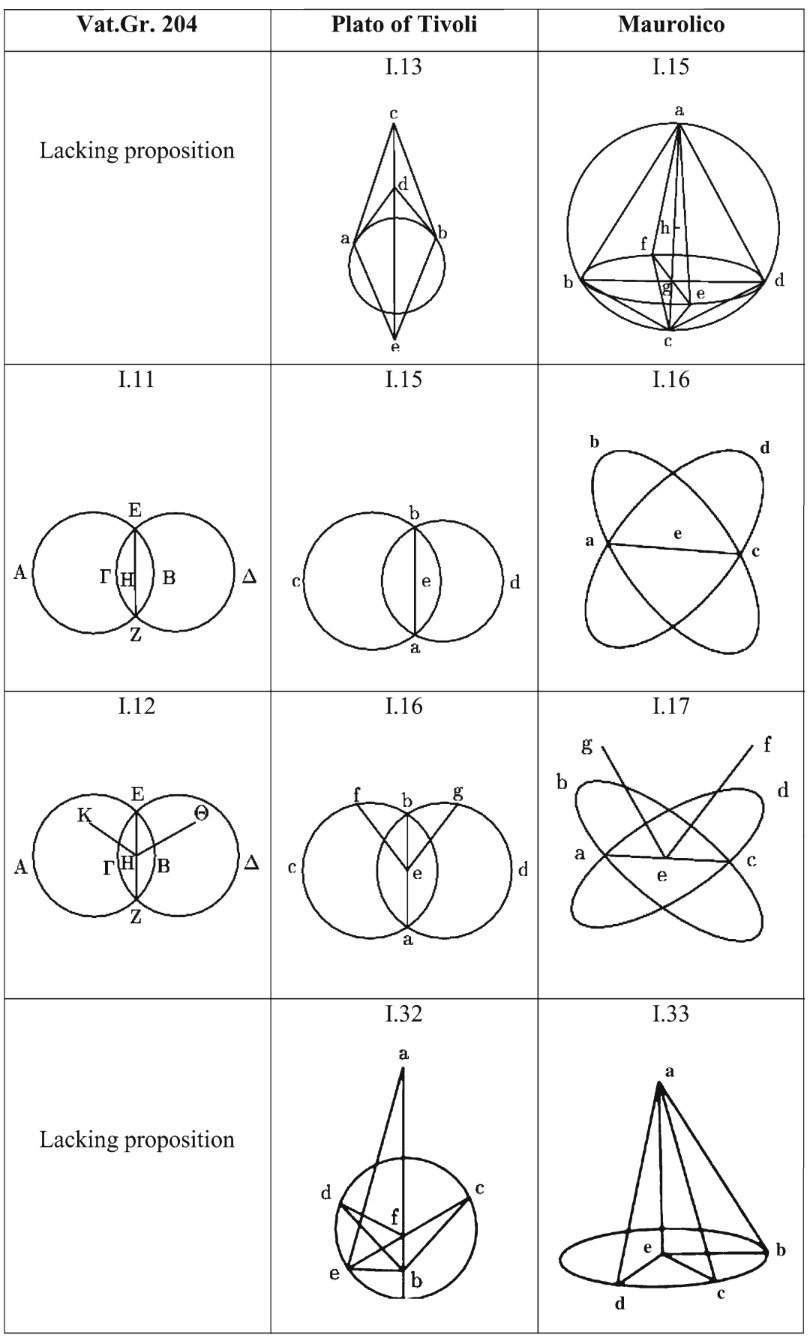
\includegraphics[width=0.9\linewidth]{images/conventions_diagrammes.png}
	\caption{Différentes conventions de représentation de diagrammes évoquées par Michela Malpangotto\footcite{malpangottoGraphicalChoicesGeometrical2010}}
	\label{fig:conventions}
\end{figure}


L'étude de Michela Malpangotto nous montre l'existence de nombreuses conventions graphiques de diagrammes pouvant être très différentes en fonction des éditeurs et des époques. Lorsque nous tentons de retracer la diffusion d'une œuvre à partir de ces diagrammes, il est important de prendre en compte ce paramètre. Néanmoins, ces différentes manières de représenter les diagrammes sont aussi en elles-mêmes les témoins de l'évolution d'un concept et donc par extension des connaissances scientifiques. \\

La question de la représentation des diagrammes est aussi une problématique que nous retrouvons dans les éditions plus contemporaines. 

\subsection{La modification des diagrammes dans les éditions modernes des sources scientifiques}

Les modifications que s'autorisent à faire les historiens et éditeurs contemporains peuvent rendre la comparaison avec les sources anciennes compliquée. Dans l'article déjà cité précédemment, Ken Saito étudie les éditions modernes des diagrammes astronomiques des \textit{Elements} d'Euclide. Il expose la problématique suivante : les diagrammes que nous voyons dans les éditions imprimées à partir du XIXe siècle sont très différents de ceux présents dans les manuscrits médiévaux. Pourtant les témoins datant du Moyen Age sont les meilleures versions, voire les seuls exemplaires d'œuvres antiques mathématiques en absence de manuscrit datant de cette époque. La version qui sert de base à beaucoup d'éditions contemporaines est celle de Heiberg datant de 1883-1888. Cependant, ce dernier s'est contenté de recopier les diagrammes de Ferdinand August simplifiés dans un but pédagogique dans son édition datant des années 1820 \footcite{saitoTraditionsDiagramTradition2012}. Se pose alors la question des conventions d'édition. Deux points de vue s'opposent. Nous avons d'abord celui de la maison d'édition \textit{Les Belles Lettres} décrit dans leur \textit{Règles et recommandations pour les éditions critiques} qui explique qu'il est nécessaire de reproduire les diagrammes aussi précisément que possible sans essayer de les corriger ou de les modifier. Michael Hunter, lui, défend plutôt l'idée selon laquelle il est acceptable que les diagrammes soient redessinés pour que l'intention originelle de l'auteur soit transmise au lecteur\footcite{jardineCriticalEditingEarlyModern2010}.\\

Ces différentes manières de représenter un même diagramme peuvent poser problème aux chercheurs lorsque ces derniers cherchent à établir des liens entre les différents témoins d'une même œuvre ou tradition. Même pour un spécialiste qui connaît parfaitement les différentes conventions, identifier et comparer chaque diagrammes dans plusieurs témoins peut s'avérer très chronophage.